% Kugelkondensator: Querschnitt mit Gauß-Kugel und Verlauf E_r(r)
% Gemeinsamer Stil für alle Abbildungen (TikZ -> SVG, siehe figures/build.mjs).
%
% Farben sind Platzhalter ("Sentinels"): build.mjs ersetzt sie im SVG durch
% CSS-Variablen, damit die Abbildungen im hellen und dunklen Modus passen.
% Andere Farben (auch schwarz/weiß) bricht der Build mit Fehler ab.
%
%   fg    Linien, Beschriftung          -> --dark
%   mu    Hilfslinien, Achsen, Maße      -> --gray
%   acc   das eine Konzept der Abbildung -> --secondary (Lime/Oliv)
%   blue  zweite Größe, negative Ladung  -> --fig-blue
%   warm  dritte Größe, positive Ladung  -> --fig-warm
%   bg    Seitenhintergrund (Aussparen)  -> --light
%
% Kein \clip verwenden: pdftocairo macht daraus Clip-Gruppen, in denen exakt
% waagerechte/senkrechte Linien verschwinden. Berechnete Kurven schneidet
% gen/*.py selbst am Rahmen ab.
\documentclass[tikz,border=3pt]{standalone}
\usepackage{amsmath,amssymb,bm}
% Text serifenlos wie die Seite, Mathe in Computer Modern wie KaTeX
\renewcommand{\familydefault}{\sfdefault}
\usetikzlibrary{arrows.meta,calc,decorations.markings,patterns,3d,positioning,angles,quotes}

\definecolor{fg}{RGB}{1,2,3}
\definecolor{mu}{RGB}{4,5,6}
\definecolor{acc}{RGB}{7,8,9}
\definecolor{blue}{RGB}{10,11,12}
\definecolor{warm}{RGB}{13,14,15}
\definecolor{bg}{RGB}{16,17,18}

% Vektoren wie auf der Website (KaTeX \mathbf)
\newcommand{\vv}[1]{\mathbf{#1}}

\tikzset{
  every picture/.style={fg, line width=0.8pt, line cap=round, line join=round,
    >={Stealth[length=5.5pt,width=4.4pt]}},
  every node/.style={font=\small},
  % Linientypen
  main/.style={line width=0.9pt},
  thin/.style={line width=0.5pt},
  aux/.style={mu, line width=0.5pt, dash pattern=on 2.5pt off 2pt},
  axis/.style={mu, line width=0.6pt, ->},
  vec/.style={line width=1.1pt, ->},
  field/.style={line width=0.7pt, postaction={decorate},
    decoration={markings, mark=at position #1 with {\arrow{Stealth[length=4.5pt,width=3.6pt]}}}},
  field/.default=0.5,
  % Flächen
  soft/.style={fill=#1, fill opacity=0.14},
  soft/.default=acc,
  % Ladungen
  qpos/.style={circle, fill=warm, inner sep=0pt, minimum size=9pt,
    path picture={\draw[bg, line width=0.9pt] ($(path picture bounding box.center)+(-2pt,0)$) -- +(4pt,0)
      ($(path picture bounding box.center)+(0,-2pt)$) -- +(0,4pt);}},
  qneg/.style={circle, fill=blue, inner sep=0pt, minimum size=9pt,
    path picture={\draw[bg, line width=0.9pt] ($(path picture bounding box.center)+(-2pt,0)$) -- +(4pt,0);}},
  dot/.style={circle, fill=fg, inner sep=0pt, minimum size=3pt},
  % Beschriftung mit Aussparung, damit Linien den Text nicht kreuzen
  lbl/.style={fill=bg, inner sep=1.5pt},
  % Icons: kräftigere Linien, keine Schrift
  icon/.style={line width=1.6pt, >={Stealth[length=6pt,width=5pt]}},
}

\begin{document}
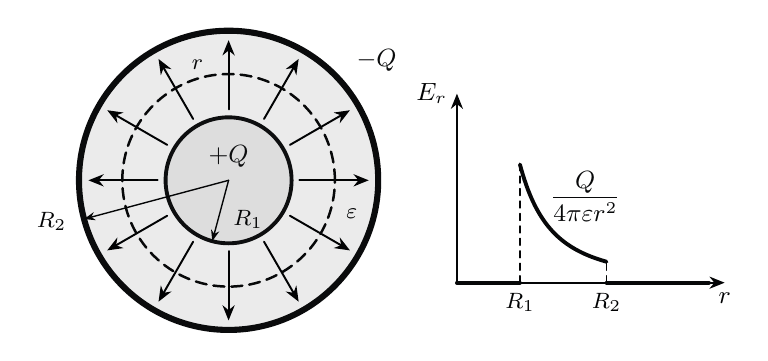
\begin{tikzpicture}
  \def\Ra{0.8}  % R_1
  \def\Rb{1.9}  % R_2
  % Dielektrikum zwischen den Kugeln
  \fill[mu, fill opacity=0.08, even odd rule] (0,0) circle (\Rb) (0,0) circle (\Ra);
  % radiales Feld
  \foreach \w in {0,30,...,330} \draw[vec, line width=0.7pt] (\w:\Ra+0.1) -- (\w:\Rb-0.12);
  % Gauß-Kugel
  \draw[acc, main, dash pattern=on 4pt off 2.5pt] (0,0) circle (1.35);
  % Elektroden
  \draw[warm, soft=warm, line width=1.4pt] (0,0) circle (\Ra);
  \draw[blue, line width=2.2pt] (0,0) circle (\Rb);
  \node[warm] at (0,0.3) {$+Q$};
  \node[blue, anchor=south west] at (40:\Rb+0.05) {$-Q$};
  % Maße in den Lücken zwischen den Feldpfeilen (alle 30°)
  \draw[thin, mu, -{Stealth[length=4pt]}] (0,0) -- (195:\Rb);
  \node[font=\footnotesize, text=mu, anchor=east] at (195:2.0) {$R_2$};
  \draw[thin, mu, -{Stealth[length=4pt]}] (0,0) -- (255:\Ra);
  \node[font=\footnotesize, text=mu, anchor=west] at (262:0.5) {$R_1$};
  \node[acc, font=\footnotesize] at (105:1.52) {$r$};
  \node[mu, font=\footnotesize] at (-15:1.62) {$\varepsilon$};

  % Verlauf E_r(r)
  \begin{scope}[xshift=2.9cm, yshift=-1.3cm]
    \def\s{0.62} % Skalierung E: E_r = s / r^2, bei R_1 = 0.97
    \draw[axis] (0,0) -- (3.4,0) node[anchor=north, text=fg] {$r$};
    \draw[axis] (0,0) -- (0,2.4) node[anchor=east, text=fg] {$E_r$};
    \draw[acc, line width=1.4pt] (0,0) -- (\Ra,0);
    \draw[acc, line width=1.4pt, domain=\Ra:\Rb, samples=60] plot (\x,{\s/(\x*\x)*1.55});
    \draw[acc, line width=1.4pt] (\Rb,0) -- (3.2,0);
    \draw[aux] (\Ra,0) -- (\Ra,{\s/(\Ra*\Ra)*1.55});
    \draw[aux] (\Rb,0) -- (\Rb,{\s/(\Rb*\Rb)*1.55});
    \node[anchor=north, font=\footnotesize] at (\Ra,0) {$R_1$};
    \node[anchor=north, font=\footnotesize] at (\Rb,0) {$R_2$};
    \node[acc, anchor=west] at (1.05,1.1) {$\dfrac{Q}{4\pi\varepsilon r^2}$};
  \end{scope}
\end{tikzpicture}
\end{document}
